\def\year{2019}\relax
\documentclass[letterpaper]{article} % DO NOT CHANGE THIS
\usepackage{aaai19}  % DO NOT CHANGE THIS
\usepackage{times}  % DO NOT CHANGE THIS
\usepackage{helvet} % DO NOT CHANGE THIS
\usepackage{courier}  % DO NOT CHANGE THIS
\usepackage[hyphens]{url}  % DO NOT CHANGE THIS
\usepackage{graphicx} % DO NOT CHANGE THIS
\urlstyle{rm} % DO NOT CHANGE THIS
\def\UrlFont{\rm}  % DO NOT CHANGE THIS
\usepackage{graphicx}  % DO NOT CHANGE THIS
\frenchspacing  % DO NOT CHANGE THIS
\setlength{\pdfpagewidth}{8.5in}  % DO NOT CHANGE THIS
\setlength{\pdfpageheight}{11in}  % DO NOT CHANGE THIS
\usepackage{amsmath, amssymb}
\graphicspath{{images/}}
\nocopyright
\usepackage{array}
\usepackage{caption}
\usepackage{xcolor}
\usepackage[outputdir=output]{minted}
\usepackage{changepage}
%PDF Info Is REQUIRED.
% For /Author, add all authors within the parentheses, separated by commas. No accents or commands.
% For /Title, add Title in Mixed Case. No accents or commands. Retain the parentheses.
\pdfinfo{
/Title (Logistic Regression)
/Author (Mark Wesley Harris)
} %Leave this	
% /Title ()
% Put your actual complete title (no codes, scripts, shortcuts, or LaTeX commands) within the parentheses in mixed case
% Leave the space between \Title and the beginning parenthesis alone
% /Author ()
% Put your actual complete list of authors (no codes, scripts, shortcuts, or LaTeX commands) within the parentheses in mixed case. 
% Each author should be only by a comma. If the name contains accents, remove them. If there are any LaTeX commands, 
% remove them. 

% DISALLOWED PACKAGES
% \usepackage{authblk} -- This package is specifically forbidden
% \usepackage{balance} -- This package is specifically forbidden
% \usepackage{caption} -- This package is specifically forbidden
% \usepackage{color (if used in text)
% \usepackage{CJK} -- This package is specifically forbidden
% \usepackage{float} -- This package is specifically forbidden
% \usepackage{flushend} -- This package is specifically forbidden
% \usepackage{fontenc} -- This package is specifically forbidden
% \usepackage{fullpage} -- This package is specifically forbidden
% \usepackage{geometry} -- This package is specifically forbidden
% \usepackage{grffile} -- This package is specifically forbidden
% \usepackage{hyperref} -- This package is specifically forbidden
% \usepackage{navigator} -- This package is specifically forbidden
% (or any other package that embeds links such as navigator or hyperref)
% \indentfirst} -- This package is specifically forbidden
% \layout} -- This package is specifically forbidden
% \multicol} -- This package is specifically forbidden
% \nameref} -- This package is specifically forbidden
% \natbib} -- This package is specifically forbidden -- use the following workaround:
% \usepackage{savetrees} -- This package is specifically forbidden
% \usepackage{setspace} -- This package is specifically forbidden
% \usepackage{stfloats} -- This package is specifically forbidden
% \usepackage{tabu} -- This package is specifically forbidden
% \usepackage{titlesec} -- This package is specifically forbidden
% \usepackage{tocbibind} -- This package is specifically forbidden
% \usepackage{ulem} -- This package is specifically forbidden
% \usepackage{wrapfig} -- This package is specifically forbidden
% DISALLOWED COMMANDS
% \nocopyright -- Your paper will not be published if you use this command
% \addtolength -- This command may not be used
% \balance -- This command may not be used
% \baselinestretch -- Your paper will not be published if you use this command
% \clearpage -- No page breaks of any kind may be used for the final version of your paper
% \columnsep -- This command may not be used
% \newpage -- No page breaks of any kind may be used for the final version of your paper
% \pagebreak -- No page breaks of any kind may be used for the final version of your paperr
% \pagestyle -- This command may not be used
% \tiny -- This is not an acceptable font size.
% \vspace{- -- No negative value may be used in proximity of a caption, figure, table, section, subsection, subsubsection, or reference
% \vskip{- -- No negative value may be used to alter spacing above or below a caption, figure, table, section, subsection, subsubsection, or reference

\setcounter{secnumdepth}{0} %May be changed to 1 or 2 if section numbers are desired.

% The file aaai19.sty is the style file for AAAI Press 
% proceedings, working notes, and technical reports.
%
\setlength\titlebox{2.5in} % If your paper contains an overfull \vbox too high warning at the beginning of the document, use this
% command to correct it. You may not alter the value below 2.5 in
\title{Logistic Regression}
%Your title must be in mixed case, not sentence case. 
% That means all verbs (including short verbs like be, is, using,and go), 
% nouns, adverbs, adjectives should be capitalized, including both words in hyphenated terms, while
% articles, conjunctions, and prepositions are lower case unless they
% directly follow a colon or long dash
\author{Mark Wesley Harris\\ % All authors must be in the same font size and format. Use \Large and \textbf to achieve this result when breaking a line
% If you have multiple authors and multiple affiliations
% use superscripts in text and roman font to identify them. For example, Sunil Issar,\textsuperscript{\rm 2} J. Scott Penberthy\textsuperscript{\rm 3} George Ferguson,\textsuperscript{\rm 4} Hans Guesgen\textsuperscript{\rm 5}. Note that the comma should be placed BEFORE the superscript for optimum readability
University of Colorado Colorado Springs\\
wharris2@uccs.edu % email address must be in roman text type, not monospace or sans serif
}
\begin{document}

\maketitle

\section{Introduction}
We previously studied how
linear regression can be used
to fit a hyperplane over feature variables of a dataset;
the goal of linear regression is to create a model capable of making a prediction for unseen input.
The same method can be applied to binary classification,
where points on one side of the hyperplane are predicted to belong to one of two classes,
and those on the opposite side are predicted to belong to the other.
While linear classification techniques work well for some distributions of data,
there are many regression problems that
cannot be solved using the step function as a separator.
%This means a higher-order
%function (or combination of functions) must be used in classification on the dataset.
%Standard linear regression methods cannot be used in classification of
%non-linearly separable data.
%However,
%To help solve more complex problems,
To combat this problem, researchers developed logistic regression.
%classify a subset of these complex problems.
%The use of the logistic function to classify non-linearly separable datasets
%is known as logistic regression.
Here we study two different ways to implement logistic regression,
the first using Gradient Ascent and the second applying the Newton-Raphson Method.
The results of our programs are evaluated against implementations using libraries in Python and R.

\section{Logistic Regression}
\begin{figure}[htbp]
\centerline{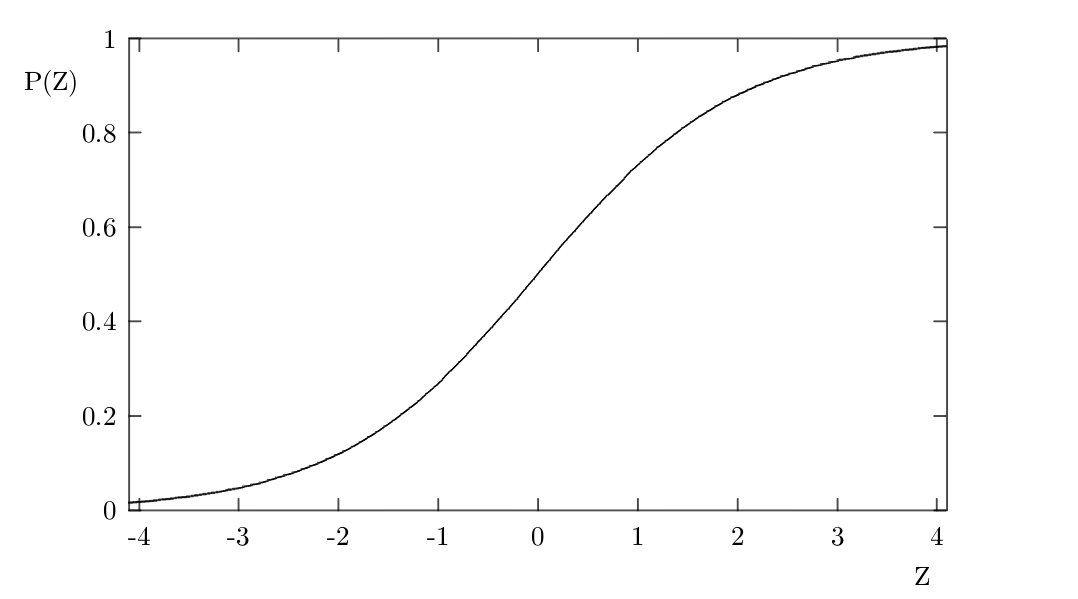
\includegraphics[width=8cm]{sigmoid.png}}
\caption{An example of the logistic curve $P(Z)$
\cite{origins}.}
\label{fig:sigmoid}
\end{figure}

The logistic function was first applied in the late 1800's
to many problems in fields such as Mathematics and Chemistry
\cite{origins}.
Transitions between one class and another are much smoother,
as is demonstrated by Figure \ref{fig:sigmoid},
By replacing the step function using in linear regression with a sigmoidal curve,
linear models became more powerful, and thus able to solve more complex problems.
%we are able to predict the probability of an element belonging to
%class 0 or class 1.
%There is a problem, however, with using this method of classification;
%most of the dataset will have either very high (class 1) or very low (class 0)
%probabilities, making training difficult.

\subsection{Logistic Fit}
The goal in logistic regression is to fit a linear combination of features and coefficients
%to predict the dependent variable
mapped to a logistic curve, rather than a step function.
%The equation of the linear function that is fitted in logistic regression
%is a linear combination of features and coefficients.
The features and coefficients are written as
$\mathbf{x}$ and $\mathbf{\theta}$, respectively.
In order to simplify our calculations, we let $x^{(0)} = 1$
and represent the combination as the inner product.

$$\mathbf{x \cdot \theta} = \theta^{(0)}x^{(0)} + \theta^{(1)}x^{(1)} + \dots + \theta^{(n)}x^{(n)}$$

Our goal is to find all coefficients,
$\theta^{(0)},\theta^{(1)},\dots,\theta^{(n)}$,
that best fit the log-odds of the dataset.
A definition of log-odds
is included later during the discussion on the objective function.

\subsection{Likelihood}
%(2)
We use the ``maximum likelihood approach'',
instead of least squared error when evaluating a logistic regression classifier.
Maximized likelihood is used widely for many Generalized Linear Models (GLM's),
and can provide ``\dots not only estimates of the regression coefficients but also
estimated asymptotic standard errors of the coefficients'' \cite{applied}.

Likelihood can be thought of as the probability that a model will correctly
predict an outcome for any input.
In the case of binary classification, the prediction belongs to one of two classes: 0 and 1.
%The likelihood is a combination of the probability
%that the outcome is predicted correctly by the model.
Recall that the standard expression used to describe conditional probability
of $Y$ given $X$ is $P(Y|X)$.
%Below is defined a
Then, using the laws of statistics, a
probability mass function can be written to express likelihood.
Here we assume that $P(Y = 1 | X = \mathbf{x}) = p(\mathbf{x};\theta)$;
thus, $p$ is a function parameterized by $\theta$
which returns the conditional probability that $Y = 1$ given $X = \mathbf{x}$.

\begin{align*}
%P(Y = 1 | X = \mathbf{x}) &= \prod_{\mathbf{x} \in Y = 1}P(Y = 1 | \mathbf{x}) \\
%P(Y = 0 | X = \mathbf{x}) &= \prod_{\mathbf{x} \in Y = 0}P(Y = 0 | \mathbf{x}) \\
%&= \prod_{\mathbf{x} \in Y = 0}(1 - P(Y = 1 | \mathbf{x}))
P(Y = 1 | X = \mathbf{x}) &= p(\mathbf{x};\theta) \\
P(Y = 0 | X = \mathbf{x}) &= 1 - P(Y = 1 | X = \mathbf{x}) \\
                          &= 1 - p(\mathbf{x};\theta)
\end{align*}

Likelihood is the combined conditional probabilities for all samples, $\mathbf{x}$,
and each class.
Thus, the above expression can be combined to obtain a measure of total likelihood
for a given input.

\begin{align*}
P(Y=y|\mathbf{x};\theta) &= P(Y = 1 | X = \mathbf{x}) * P(Y = 0 | X = \mathbf{x}) \\
&= p(\mathbf{x};\theta)^y(1-p(\mathbf{x};\theta))^{y - 1}
\end{align*}

We can find the likelihood of an entire dataset, $\mathbf{D}$,
by taking the product of all likelihoods on sample $\mathbf{x} \in \mathbf{D}$,
as shown in Equation \ref{eq:probability}.
%Here $n$ is the number of Classes.
%We have two classes, 0 and 1, so $n = 2$.
%Order of the classes is inconsequential for the final product
Here $N$ represents the number of training samples,
and $\mathbf{x}_i$ and $y_i$ correspond to the input vector and output value,
respectively.
\cite{data_analysis}.

\begin{equation}
\begin{split}
\label{eq:probability}
Likelihood(\mathbf{D}) &= \prod_{i=1}^{N}P(Y=y_i|\mathbf{x}_i;\theta) \\
&= \prod_{i=1}^{N}p(\mathbf{x}_i;\theta)^{y_i}(1 - p(\mathbf{x}_i;\theta)^{1 - y_i})
\end{split}
\end{equation}

By using the properties of logarithms,
we can take the $\log$ of the likelihood and simplify as
shown in Equation \ref{eq:likelihood} \cite{data_analysis}.

\begin{equation}
\begin{split}
\label{eq:likelihood}
\log(\prod_{i = 1}^{n}p(\mathbf{x}_i;\theta)^{y_i}(1 - p(\mathbf{x}_i;\theta)^{1 - y_i})) = \\
\sum_{\mathbf{x}}[y\log(p(\mathbf{x};\theta)) + (1 - y)\log(p(\mathbf{x};\theta)))]% = \\
%y*\log\frac{p(\mathbf{x};\theta)}{1 - p(\mathbf{x};\theta)}
\end{split}
\end{equation}

The result is a transformed version of the likelihood,
where probabilities are projected into log-space.
This is referred to as log-likelihood, and is used to define the gradient
in logistic regression.

\subsection{Objective Function}
%(3)
%Derive the objective function used in logistic regression.
Our goal is to maximize the log-likelihood
by optimizing $\mathbf{\theta}$ over feature space $\mathbf{x}$.
The linear combination, $\mathbf{x\cdot\theta}$,
is fit in relation to log-odds.
This is expressed mathematically by
Equation \ref{eq:log-odds}.

\begin{equation}
\label{eq:log-odds}
\log \frac{p(\mathbf{x};\theta)}{1 - p(\mathbf{x};\theta)} = \mathbf{x \cdot \theta}
\end{equation}

We can now solve for $p$ in order to obtain the log-odds formula
\cite{data_analysis}.

\begin{equation}
\begin{split}
\label{eq:likelihood}
\log \frac{p(\mathbf{x};\theta)}{1 - p(\mathbf{x};\theta)} &= \mathbf{x \cdot \theta} \\
p(\mathbf{x};\theta) &= e^{\mathbf{x} \cdot \theta}(1 - p(\mathbf{x};\theta)) \\
&= e^{\mathbf{x} \cdot \theta} - e^{\mathbf{x} \cdot \theta}p(\mathbf{x};\theta)) \\
&= \frac{e^{\mathbf{x} \cdot \theta}}{1 + e^{\mathbf{x} \cdot \theta}} \\
&= \frac{1}{1 + e^{-\mathbf{x} \cdot \theta}}
\end{split}
\end{equation}

Thus, the objective function can be stated as: ``To find $\theta$
such that the log-likelihood is maximized.''
Equation \ref{eq:objective} expresses this statement mathematically \cite{data_analysis}.

\begin{equation}
\label{eq:objective}
%\ell(\theta) = \text{argmax}_{\theta} = \sum_{\mathbf{x}}y(\mathbf{x}\cdot\theta) + \log(1 - p(\mathbf{x};\theta))
\ell(\theta) \leftarrow \text{argmax}_{\theta} = \sum_{\mathbf{x}}y(\mathbf{x}\cdot\theta) - \log(1 + p(\mathbf{x};\theta))
\end{equation}

\subsection{Gradient Ascent}
%(4)
Recall that the gradient of a function measures the direction that the function is increasing the
fastest at the given point. Thus the gradient can be used in part of an iterative process to find
the maxima of the function.
It can be shown that the gradient of log-likelihood simplifies to Equation \ref{eq:gradient}.
Note that since we let $x^{(0)} = 1$, there is no need to specify an extra rule for the intercept coefficient,
$\theta^{(0)}$.

\begin{equation}
\label{eq:gradient}
\nabla_{\theta} = 
\sum_{i=1}^{n}[p(\mathbf{x};\theta) - y]x^{(i)}
\end{equation}

Since $p(\mathbf{x};\theta) - y$ represents a form of loss from classification,
the log-odds equation can similarly be thought of as a cost function for the fit of coefficients.
The gradient step is written below in vector form.
$\lambda$ is a learning parameter, used to ensure coefficients converge with minimal over-fitting.

$$\theta = \theta - \lambda\nabla_{\theta}$$

\subsection{Newton-Raphson Method}
%(5)
\begin{figure}[htbp]
\centerline{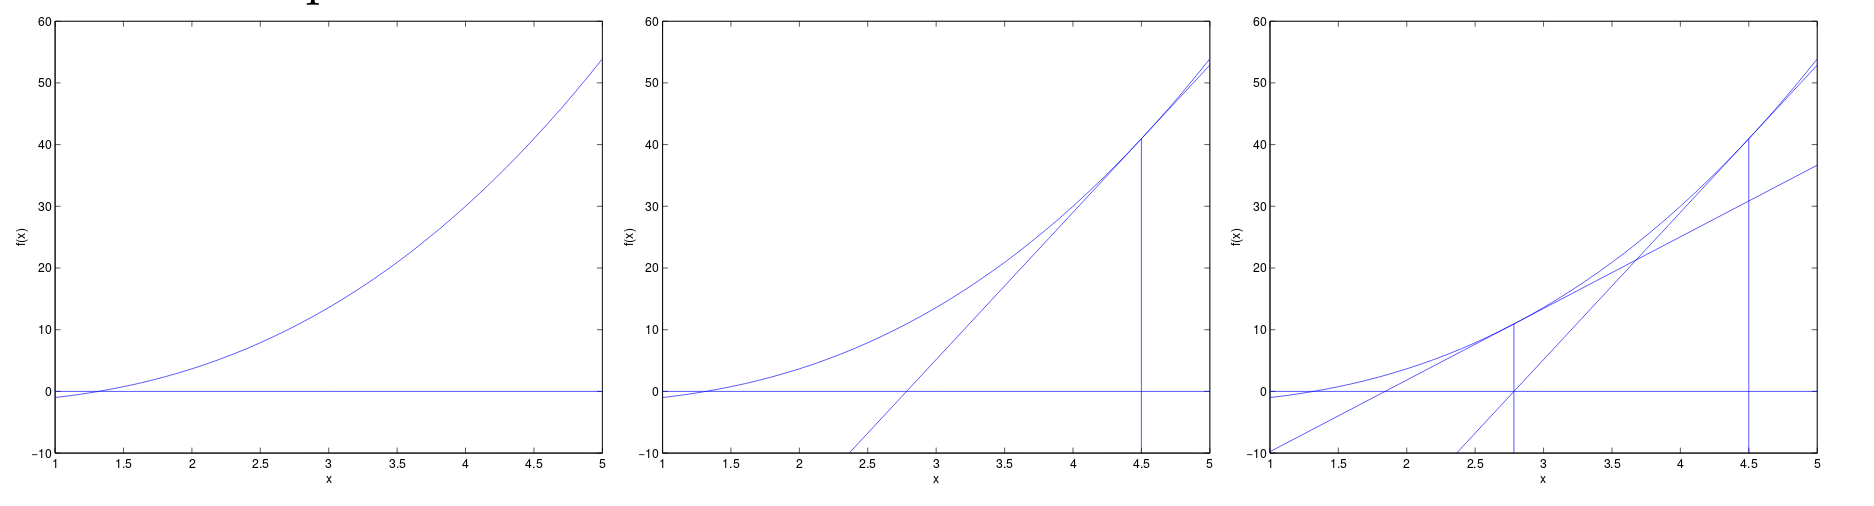
\includegraphics[width=8cm]{newton.png}}
\caption{An example of 2 iterations of the Newton-Raphson method
\cite{notes}.}
\label{fig:newton}
\end{figure}

The Newton-Raphson method -- also called Newton's method --
can be used to find the roots of a differentiable function.
The generalized method is shown in Equation \ref{eq:newton},
and a few iterations of the process are displayed in Figure \ref{fig:newton} \cite{notes}.

\begin{equation}
\label{eq:newton}
\theta_{n + 1} = \theta_n - \frac{f(\theta_n)}{f'(\theta_n)}
\end{equation}

%For logistic regression as outlined above,
%the function to evaluate in terms of $x$
%(for now we consider the non-vector case)
%is $f(x) = \frac{1}{1 + e^{-x}}$.
Applying Equation \ref{eq:newton} to our multi-dimensional feature space,
we can derive the following expression.
Note that $H^{-1}$ represents the inverse of the $n \times n$ Hessian matrix,
where $n$ is the number of feature attributes.
$\nabla_{\theta}f(\theta)$ is again the gradient of the objective function.

$$\theta_{n+1} = \theta_n - H^{-1}\nabla_{\theta}f(\theta)$$

The Hessian is a matrix of partial derivatives which serves to express
the gradient for functions that are dependent on more than one feature \cite{notes}.
It is necessary to use the Hessian
since the feature space is multi-dimensional; if there were only a single dependent variable,
the derivation would give the second derivative without needing to use the Hessian matrix.
A mathematical equation for the Hessian is produced in Equation \ref{eq:hessian} below.

\begin{equation}
\label{eq:hessian}
H_{ij} = \frac{\partial^2f(\mathbf{x};\theta)}{\partial\theta_i\partial\theta_j}
\end{equation}

To implement the Newton-Raphson method we must
find the Hessian, which involves
calculating the first and second partial derivatives of the objective function.
The steps of this derivation are shown below.

First we find $\frac{\partial f}{\partial\theta_i}$.
Here the quotient rule is applied, where $h = 1$ and $g = 1 + e^{-\mathbf{x\cdot\theta}}$.
\begin{align*}
\frac{\partial f}{\partial\theta_i} = (\frac{h}{g})' &= \frac{h'g - hg'}{g^2} \\
    &= \frac{0(1 + e^{-\mathbf{x\cdot\theta}})
       - (-1)x_ie^{-\mathbf{x\cdot\theta}}}
            {(1 + e^{-\mathbf{x\cdot\theta}})^2} \\
    &= x_i\frac{e^{-\mathbf{x\cdot\theta}}}
            {(1 + e^{-\mathbf{x\cdot\theta}})^2}
\end{align*}

The negative was taken out of the partial for simplicity.
Using the result of $\frac{\partial f}{\partial x_i}$,
we can calculate $\frac{\partial^2 f}{\partial x_i\partial x_j}$.
The same as in the previous step, we must apply the quotient rule, where
$h = \theta_ie^{-\mathbf{x\cdot\theta}}$ and
$g = (1 + e^{-\mathbf{x\cdot\theta}})^2$.

\begin{align*}
\frac{\partial^2 f}{\partial\theta_i\partial\theta_j}
    &= [-x_ix_je^{-\mathbf{x\cdot\theta}}
       (1+e^{-\mathbf{x\cdot\theta}})^2 \\
    &+ 2x_ix_je^{-2\mathbf{x\cdot\theta}}
    (1+e^{-\mathbf{x\cdot\theta}})] / (1 + e^{-\mathbf{x}\cdot\theta})^4 \\
    &= (1 + e^{-\mathbf{x}\cdot\theta})
    [-x_ix_je^{-\mathbf{x}\cdot\theta}(1 + e^{-\mathbf{x}\cdot\theta}) \\
    &+ 2x_ix_je^{-2\mathbf{x}\cdot\theta}]
    / (1 + e^{-\mathbf{x}\cdot\theta})^4 \\
    &= x_ix_j\frac{e^{-2\mathbf{x}\cdot\theta} - e^{-\mathbf{x}\cdot\theta}}
       {(1 + e^{-\mathbf{x}\cdot\theta})^3}
\end{align*}

This kind of simplification is possible since the expression
$\mathbf{x}\cdot\theta$ is a linear combination of parameters and feature values,
and because to the simplicity of exponential differentiation.
If $p(\mathbf{x};\theta)$ did not have both of these properties,
it is unlikely we would obtain such a simplified answer.
%Equation \ref{eq:hessian_expand}
The final Hessian matrix used in the Newton-Raphson method is expressed below,
where
$
\psi = \frac{e^{-2\mathbf{x}\cdot\theta} - e^{-\mathbf{x}\cdot\theta}}
{(1 + e^{-\mathbf{x}\cdot\theta})^3}
$
and $\sum$ represents the summation of all samples $\mathbf{x}$ in dataset $\mathbf{D}$
(these substitutions serve only to shorten the representation for the matrix).

\small
$$
H(p(\mathbf{x};\theta)) =
\begin{bmatrix}
\sum\psi & \sum\mathbf{x}_1\psi & \sum\mathbf{x}_2\psi & \sum\mathbf{x}_3\psi\\
\sum\mathbf{x}_1\psi  &  \sum\mathbf{x}_1^2\psi  &  \sum\mathbf{x}_1\mathbf{x}_2\psi  &  \sum\mathbf{x}_1\mathbf{x}_3\psi\\
\sum\mathbf{x}_2\psi  &  \sum\mathbf{x}_1\mathbf{x}_2\psi  &  \sum\mathbf{x}_2^2\psi  &  \sum\mathbf{x}_2\mathbf{x}_3\psi\\
\sum\mathbf{x}_3\psi  &  \sum\mathbf{x}_1\mathbf{x}_3\psi  &  \sum\mathbf{x}_2\mathbf{x}_3\psi  &  \sum\mathbf{x}_3^2\psi\\
\end{bmatrix}
$$
\normalsize

\section{Implementation}
The dataset chosen for classification was
the Skin Segmentation dataset from UCI Machine Repository.
This dataset classifies cells,
where one class represents skin cells and the other class represents non-skin cells.
The function is dependent upon the red, green, and blue color features for each cell.
Thus, the classification problem presented is to predict the class for a cell
given its RGB color. Table \ref{tbl:data} shows some samples of the dataset.
The integer values were treated as floating point values when being evaluated.

\begin{table}[t]
\begin{centering}
\bgroup
\def\arraystretch{1.5}
\begin{tabular}{| m{0.0925\textwidth} | m{0.0925\textwidth} | m{0.0925\textwidth} | m{0.0925\textwidth} |} 
\hline
$B$ & $G$ & $R$ & $Class$ \\ 
\hline
\hline
74 & 85 & 123 & 0 \\ 
\hline
73 & 84 & 122 & 0 \\ 
\hline
\ldots & \ldots & \ldots & \ldots \\ 
\hline
163 & 162 & 112 & 1 \\ 
\hline
255 & 255 & 255 & 1 \\ 
\hline
\end{tabular}
\caption{Samples from the Skin Segmentation dataset \cite{skin}.}
\label{tbl:data}
\egroup
\end{centering}
\end{table}

\subsection{Implementation Details}
Stochastic Gradient Ascent and the Newton-Raphson method were implemented
in order to train two different logistic regression models.
A pair of library implementations was also created, to help in evaluation.
The Logistic Regression package from Scikit Learn Python library was used 
for the Python implementation \cite{python}.
Similarly, the Logistic Regression function from the GLM library was used
for the R program \cite{r}.

Several challenges were overcome during program implementation.
The complexity of the Hessian was an expected hurdle, however it took longer
than expected to produce a working regression model using the Newton-Raphson method.
There was also some confusion regarding the equations for the gradient and Hessian,
which was resolved after realizing that they involved sums over the entire dataset
as opposed to working with single elements, like with linear regression.
Finally, the selected dataset was very large (with over 200,000 entries), which added processing time
to every change in the code.

\subsection{Evaluation}
Logistic regression cannot be evaluated in the same way as linear regression,
since we are maximizing log-likelihood instead of minimizing squared error.
Therefore, $R^2$ is not an applicable evaluation criteria for these models.
Instead, we must compare the performance of classification over set of test data
that was not used in training the model.
Accuracy was found to be an apt mode of evaluation;
accuracy of a trained model by using the simple formula below.

$$\text{Accuracy} = \frac{\text{Number of correct predictions}}{\text{Number of total predictions}}$$

This ratio gives us the percentage of the time the model makes a correct classification given input features.
In order to fairly evaluate the predictiveness of each model,
25\% of the Skin Segmentation dataset was used for testing and the remaining 75\% was used for training.
Accuracies for each model are recorded in Table \ref{tbl:accuracy}.

\section{Results}
In theory, one notable difference between the gradient and Newton-Raphson methods of updating coefficients
is the time taken until convergence.
As a trade-off, the Newton-Raphson method can take significantly longer to compute for
a large number of attributes, since the Hessian is an $n \times n$ matrix.
Our implementations did not prove the first claim.
However, since hyper-parameters were not fine tuned
for either model, further investigation on performance is necessary.
%As shown in Figure \ref{fig:converge}, SGD takes a longer time to converge on average
%compared to the Newton-Raphson method.
For instance, setting the learning parameter of the gradient model to $0.01$
resulted in an accuracy of $0.778324$, which is a drop of around $-0.126$.
While the experiment led to poor predictions, the iterations decreased by $78$
before convergence, meaning the algorithm ran many times faster.
We can see from this how important it is to find the perfect learning parameter
for training, which is why the library implementations find
optimized parameters for their calculations and run very fast in comparison.

\begin{table}[t]
\begin{centering}
\bgroup
\def\arraystretch{1.5}
\begin{tabular}{| m{0.17\textwidth} | m{0.254\textwidth} |} 
\hline
Method & Fit \\ 
\hline
\hline
Our Python Gradient & $0.000626 - 0.023371B + 0.010605G - 0.023756R$ \\
\hline
Our Python Newton's & $0.694826 - 0.005322B - 0.001088G - 0.006400R$ \\
\hline
\hline
Library Python & $4.58772208 + 0.02863928B - 0.0116474G - 0.03371963R$ \\
\hline
Library R & $4.5880801 + 0.0286520B - 0.0116430G - 0.0337475R$ \\
\hline
\end{tabular}
\caption{Fits found for each model.}
\label{tbl:fits}
\egroup
\end{centering}
\end{table}

The fits between ours and the library implementations are slightly different,
however the evaluation of the models proves that the coefficients were properly
optimized. Concerning accuracies of the gradient and Newton-Raphson models,
there were only slightly off from the library implementations.
Although our implementations ran much slower and with more iterations,
the models gave the same quality of accuracy when predicting on new data.

Both library models have good accuracy, and it is clear that either would do a good job in
evaluating new data. However, it was noted that the R program executed much quicker than the Python program
for all runs.
The bottleneck was found to be in the data import function called for the Python
implementation. If this were to be replaced with an importer as efficient as
the R program, then both implementations would be comparable in performance
and accuracy.

\begin{table}[t]
\begin{centering}
\bgroup
\def\arraystretch{1.5}
\begin{tabular}{| m{0.17\textwidth} | m{0.12\textwidth} | m{0.12\textwidth} |} 
\hline
Method & Accuracy & Iterations \\ 
\hline
\hline
Our Python Gradient & $0.904366$ & $85$ \\
\hline
Our Python Newton's & $0.924247$ & $100$ \\
\hline
\hline
Library Python & $0.917449$ & $14$ \\
\hline
Library R & $0.920443$ & $6$ \\
\hline
\end{tabular}
\caption{Accuracies and number of iterations for each model.}
\label{tbl:accuracy}
\egroup
\end{centering}
\end{table}

\section{Conclusion}
We successfully showed that logistic regression models
maximizing log-likelihood
can be implemented
using gradient and Newton-Raphson methods.
The fits, accuracies, and statistics for each model were collected and evaluated.
We found that our implementations, although slower and less efficient,
were just as accurate as the standard library implementations.
Our analysis shows that logistic regression models are
suitable to solve more complex problems than with regular linear regression.
While not all problems are well-suited for linear regression, linear techniques
can still be used to obtain good predictions for complex problems.

\bibliography{report}
\bibliographystyle{aaai}

\onecolumn

\pagebreak

\begin{center}
\section*{Appendix}
\label{app:b}
\end{center}

\bigskip

\footnotesize{
\begin{minted}{python}
# sgd.py

import math as math
import pandas as pd
import numpy as np
import utilities

# Definition of Stochastic Gradient Descent algorithm.
def model(x, y, max_epochs, epsilon, beta):
    # Initialize variables.
    coeffs = np.zeros(x.shape[1])
    l_delta = epsilon + 1
    l_curr = 0
    epochs = 0

    while epochs < max_epochs and l_delta > epsilon:
        # Find gradient.
        grad = utilities.gradient(y, x, coeffs)
        print(grad)

        # Update step.
        coeffs -= beta * grad.A1
        predictions = utilities.get_predictions(x, coeffs)
        l_calc = utilities.loss(y, predictions)
        l_delta = np.abs(l_calc - l_curr)
        l_curr = l_calc
        epochs += 1

        #print('Coeffs: ', coeffs)
        print('%d.\tLoss: %0.06f' % (epochs, l_calc))
        #print('Loss Deltas: ', l_delta)

    return coeffs
\end{minted}

\bigskip

\begin{minted}{python}
# newton.py

import math as math
import pandas as pd
import numpy as np
import utilities

# Define method for calculating Newton-Raphson value(s).
def model(x, y, max_epochs, epsilon, beta):
    # Initialize variables.
    coeffs = np.zeros(x.shape[1])
    l_delta = epsilon + 1
    l_curr = 0
    epochs = 0

    while epochs < max_epochs and l_delta > epsilon:
        # Find the gradient and Hessian using current coefficients.
        grad = utilities.gradient(y, x, coeffs)
        hess = utilities.hessian_matrix(x, coeffs)
        try:
            hess = np.linalg.inv(hess)
        except:
            hess = np.identity(len(x[0]), dtype=float)

        # Update step.
        step = np.dot(hess, grad.T)
        #print('Update Step: ', step.A1)
        for i in range(len(coeffs)):
            if epochs == 0:
                coeffs[i] = step[i]
            else:
                coeffs[i] = coeffs[i] - beta * step[i]

        predictions = utilities.get_predictions(x, coeffs)
        l_calc = utilities.loss(y, predictions)
        l_delta = np.abs(l_calc - l_curr)
        l_curr = l_calc
        epochs += 1

        #print('Coeffs: ', coeffs)
        print('%d.\tLoss: %0.06f' % (epochs, l_calc))
        #print('Loss Deltas: ', l_delta)

    return coeffs

\end{minted}

\bigskip

\begin{minted}{python}
# stats.py

import math as math
import pandas as pd
import numpy as np
import utilities
import sgd
import newton

# Define method for evaluating the fit of a model.
def evaluate_model(x, y, coeffs):
    correct = 0
    incorrect = 0
    predictions = utilities.get_predictions(x, coeffs)

    for i in range(len(predictions)):
        # Correct prediction.
        if (y[i] == 0 and predictions[i] < 0.5) or (y[i] == 1 and predictions[i] >= 0.5):
            correct += 1
        # Incorrect prediction.
        else:
            incorrect += 1

    print('Accuracy: %0.06f' % (correct / float(correct + incorrect)))

# Import dataset.
dataset = utilities.import_SS(False)

# Split dataset into training and test data.
x_data = dataset.iloc[:,0:3]
y_data = dataset.iloc[:,3]
offset = int(x_data.shape[0] * 0.75)
x_train, y_train = x_data[:offset], y_data[:offset]
x_test, y_test = x_data[offset:], y_data[offset:]

# Get samples.
x, y = utilities.get_samples(x_train, y_train)

# Format:
# *.model(X, y, max_epochs, epsilon, beta (learning parameter))

coeffs = sgd.model(x, y, 100, 0.0001, 0.001)
print('SGD Stats...')
print(coeffs)
x, y = utilities.get_samples(x_test, y_test)
evaluate_model(x, y, coeffs)

# Get samples.
x, y = utilities.get_samples(x_train, y_train)

coeffs = newton.model(x, y, 100, 0.0001, 0.01)
print('Newton Stats:')
print(coeffs)
x, y = utilities.get_samples(x_test, y_test)
evaluate_model(x, y, coeffs)
\end{minted}

\bigskip

\begin{minted}{python}
# library.py

# Modeled off of "Logistic Regression" on SciKit Learn (Library)
# Source: https://scikit-learn.org/stable/modules/generated/sklearn.linear_model.Logistic
          Regression.html

import pandas as pd
import numpy as np
import matplotlib.pyplot as plt
import matplotlib.patches as mpatches
import utilities

from sklearn.linear_model import LogisticRegression
from sklearn.metrics import mean_squared_error

# Load dataset.
dataset = utilities.import_SS(False)
x = dataset.iloc[:,0:3]
y = dataset.iloc[:,3]
offset = int(x.shape[0] * 0.9)
x_train, y_train = x[:offset], y[:offset]
x_test, y_test = x[offset:], y[offset:]

# Fit regression model.
model = LogisticRegression()
fit = model.fit(x_train, y_train)
predictions = model.predict(x_test)

# Print stats
print(model.score(x_test, y_test))
print(model.intercept_, model.coef_)
print(model.n_iter_)
\end{minted}

\bigskip

\begin{minted}{r}
# library.r

# Modeled off of "Extreme Gradient Boosting (XGBoost) with R and Python"
# Source: https://datascience-enthusiast.com/R/ML_python_R_part2.html

if(!require(readxl)) install.packages("readxl", repos = "http://cran.us.r-project.org")
if(!require(xgboost)) install.packages("xgboost", repos='http://cran.rstudio.com/')
if(!require(caret)) install.packages("caret", repos='http://cran.rstudio.com/')
#if(!require(InformationValue)) install.packages("InformationValue", repos='http://cran.
                                                                         rstudio.com/')
library("readxl")
library("xgboost")
library("caret")
#library("InformationValue")

# Load and partition data.
dataset <- as.data.frame(read_excel("../../source/SkinSegmentation/SkinSegmentation.xlsx"))
partition <- createDataPartition(y = dataset$C, p = 0.75, list = FALSE)
train_data <- dataset[partition,]
test_data <- dataset[-partition,]

# Convert data into DMatrix format.
x_train = as.data.frame(train_data[1:3])
y_train = train_data$C
x_test = as.data.frame(test_data[1:3])
y_test = test_data$C

model <- glm(as.factor(C) ~ ., family=binomial(link='logit'), data=train_data)

# Calculate accuracy.
fitted.results <- predict(model,newdata=test_data,type='response')
fitted.results <- ifelse(fitted.results > 0.5,2,1)
error <- mean(fitted.results != test_data$C)
print(paste('Accuracy',1 - error))
summ <- summary(model)
print(summ)
\end{minted}
\end{document}
